The methodology will outline the systematic process used to create and evaluate the \textbf{eC-Tab2Text dataset}, which is designed to enhance the performance of Large Language Models (LLMs) in generating accurate and meaningful product reviews for e-commerce applications.
\\

This process spans from the initial data acquisition and preparation to the fine-tuning and evaluation of LLMs. Each stage is essential to ensuring that the dataset effectively bridges the gap between structured product data and user-centric textual reviews.
\\

The methodology is summarized in a flowchart (Figure \ref{fig:MethodologyFlowchart}). This structured approach guarantees a comprehensive and reproducible pathway for leveraging LLMs to transform structured product data into human-readable reviews while addressing challenges such as data sparsity and domain-specific needs.
\begin{figure}[H]
    \centering
    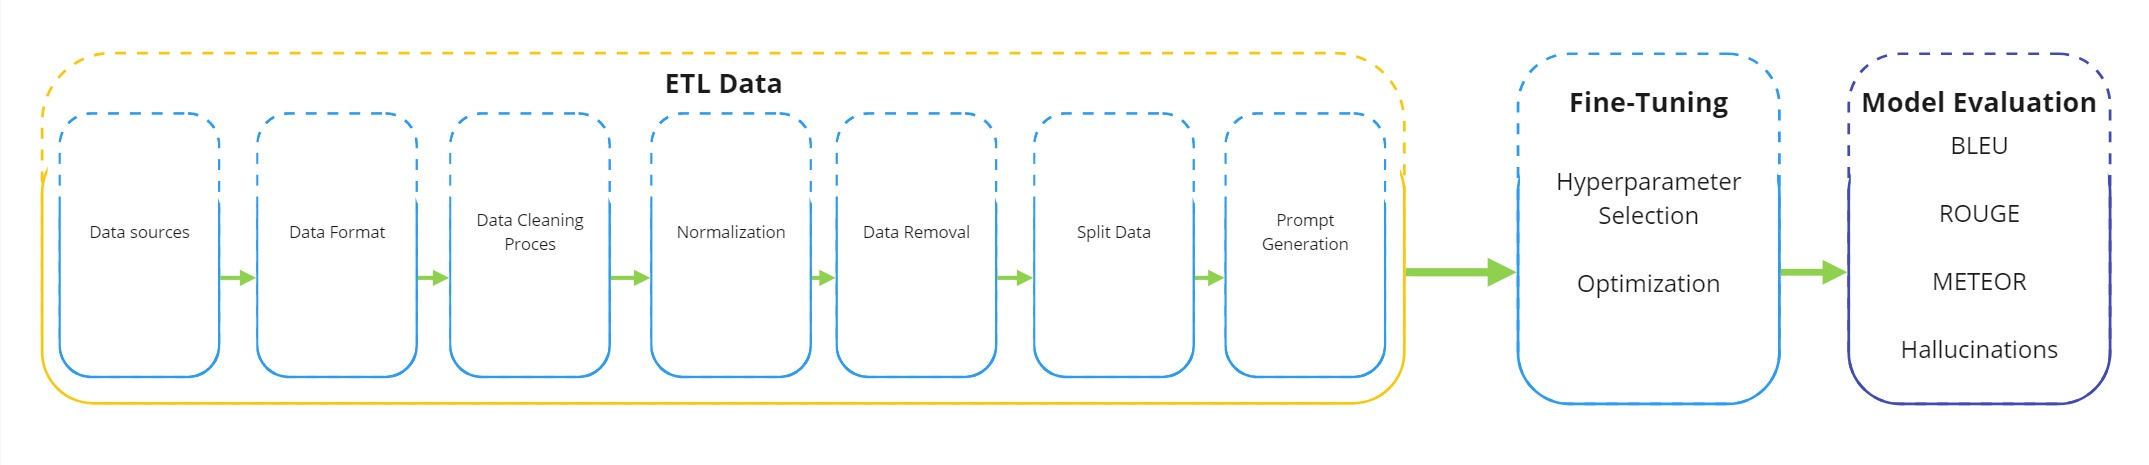
\includegraphics[width=10cm]{images/Methodology.jpg}
    \caption{Methodology Flowchart}
    \label{fig:MethodologyFlowchart}
\end{figure}
